\section[Технические подробности]{Технические подробности приготовления и измерения состояний}
Алиса активирует лазер (рис. \ref{fig:scheme}) в определенный момент времени и получает на выходе интенсивное когерентное состояние, локализованное в интервале $l_{pac}$. 
Интерферометр Алисы состоит из двух симметричных светоделителей и задержки по одному плечу между ними. В плече с задержкой также установлен фазовый модулятор, но при первом проходе он не используется и на состояния не влияет. 

Симметричный светоделитель вводится как оператор $\hat{U}_{50/50}$, действующий на два когерентных состояния на входе следующим образом:
\begin{equation}
  \hat{U}_{50/50} 
  \begin{bmatrix}
    \state{\alpha} \\
    \state{\beta}
  \end{bmatrix}
  =
  \begin{bmatrix}
    \frac{1}{\sqrt{2}}(\state{\alpha + \beta}) \\
    \frac{1}{\sqrt{2}}(\state{\alpha - \beta})
  \end{bmatrix}.
\end{equation}
То есть в один выход светоделителя направляется сумма входных состояний, в другой~--- их разность.

Если на входе светоделителя только одно состояние (второе вакуумное), то это состояние <<расщепится>> и в оба выхода светоделителя отправятся одинаковые части:
\begin{equation}
  \hat{U}_{50/50} 
  \begin{bmatrix}
    \state{\alpha} \\
    0
  \end{bmatrix}
  =
  \begin{bmatrix}
    \frac{\state{\alpha}}{\sqrt{2}} \\
    \frac{\state{\alpha}}{\sqrt{2}}
  \end{bmatrix}.
\end{equation}

Если эти <<половинки>> одновременно достигнут входа второго светоделителя, то, согласно определению, в верхний выход отправится исходное состояние \state{\alpha}, в нижнем не будет ничего:
\begin{equation}
  \hat{U}_{50/50} 
  \begin{bmatrix}
    \frac{\state{\alpha}}{\sqrt{2}} \\
    \frac{\state{\alpha}}{\sqrt{2}}
  \end{bmatrix}  
  =
  \begin{bmatrix}
    \frac{1}{\sqrt{2}} \cdot \frac{1}{\sqrt{2}}(\state{\alpha+\alpha}) \\
    \frac{1}{\sqrt{2}} \cdot \frac{1}{\sqrt{2}}(\state{\alpha-\alpha})
  \end{bmatrix}
  =
  \begin{bmatrix}
    \state{\alpha} \\
    0
  \end{bmatrix}.
\end{equation}

При прохождении через интерферометр локализованное состояние Алисы преобразуется в состояние из двух половинок, разделенных интервалом $l$: $|\alpha_c\rangle_1 \otimes |\alpha_c\rangle_2$. 
Затем состояние через линзовую систему направляется в канал связи. Приготовление протяженного состояния из локализованного требует конечного времени (рис \ref{fig:process}).

На приемной стороне Боба классическое состояние вводится в волоконную часть. 
Через светоделитель состояние поступает на классический детектор, по импульсу тока на котором оценивается интенсивность состояния и записывается его время прилета. 
Затем сигнал отражается от фарадеевского зеркала, в зависимости от сигнала на детекторе ослабляется и становится равным $|\alpha\rangle_1 \otimes |\alpha\rangle_2$.
При прохождении второй половинки ослабленного состояния через фазовый модулятор на последний подается импульс напряжения и <<навешивается>> относительная фаза.
Получившееся состояние $|\alpha\rangle_1 \otimes |e^{i\varphi_B}\alpha\rangle_2$ направляется к Алисе.

\begin{figure}[h]
\center{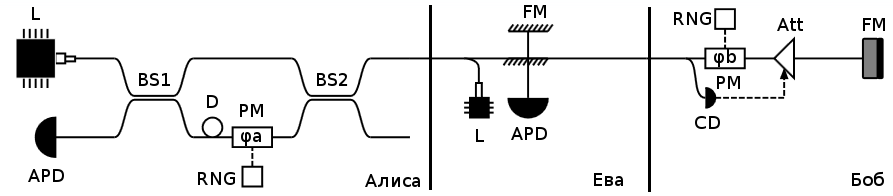
\includegraphics[width=1\linewidth]{scheme}}
\caption{
Двухпроходная оптическая схема приготовления, преобразования и детектирования состояний.
L~--- лазер, APD~--- лавинный стробируемый однофотонный детектор, BS1, BS2~---интерферометр с разностью хода по нижнему и верхнему плечу,
D~--- задержка в плече интерферометра, PM~--- фазовый модулятор, RNG~--- генератор случайных чисел,
CD~--- быстрый классический детектор, Att~--- управляемый аттенюатор, FM~--- фарадеевское зеркало
}
\label{fig:scheme}
\end{figure}

Поскольку Алиса знает время приготовления своего состояния и расстояние $L$ между передающей и приемной станциями, при обратном проходе она активирует фазовый модулятор в момент прохождения первой половины состояния по нижнему, более длинному, плечу интерферометра. 
Из-за разности хода на втором светоделителе интерферируют передняя, из нижнего плеча, и задняя, из верхнего плеча интерферометра, половинки.
Таблица \ref{tabular:transforms} отражает последовательное преобразование состояний по оптическому тракту.

\begin{table}[h]
\caption{Преобразование состояний по оптическому тракту на пути от Боба к Алисе}
\label{tabular:transforms}
\begin{center}
\begin{tabular}{|c|c|c|}
\hline
Верхний и нижний & Верхнее и нижее & Верхний и нижний \\
входы BS 	& плечо BS после PM & выход BS \\
\hline

$|\alpha \rangle_1 \otimes |e^{i\varphi_B} \alpha \rangle_2 \otimes |vac \rangle_3$ 	& 
$|\frac{\alpha}{\sqrt{2}} \rangle_1 \otimes |\frac{e^{i\varphi_B} \alpha}{\sqrt{2}} \rangle_2 \otimes |vac \rangle_3$	& 
$|\frac{\alpha}{2} \rangle_1 \otimes |\frac{(e^{i\varphi_B} + e^{i\varphi_A}) \alpha}{2} \rangle_2 \otimes |\frac{\alpha}{2} \rangle_3$ \\
\hline 

$|vac \rangle_1 \otimes |vac \rangle_2 \otimes |vac \rangle_3$ 	&
$|vac \rangle_1 \otimes |\frac{e^{i\varphi_A} \alpha}{\sqrt{2}} \rangle_2 \otimes |\frac{\alpha}{\sqrt{2}} \rangle_3$ & 
$|\frac{\alpha}{2} \rangle_1 \otimes |\frac{(e^{i\varphi_B} - e^{i\varphi_A}) \alpha}{2} \rangle_2 \otimes |\frac{\alpha}{2} \rangle_3$  \\
\hline
\end{tabular}
\end{center}
\end{table}

На входе лавинного фотодетектора в центральном временном окне 2 состояние равно $|\frac{(e^{i\varphi_B} - e^{i\varphi_A})\alpha}{2}\rangle_2$.
При обратном проходе состояния в плече лазера являются холостыми.

Далее, если Боб выбрал $\varphi_B = \varphi_0$, а Алиса выбрала также $\varphi_A = \varphi_0$ (или $\varphi_B = \varphi_1$ и $\varphi_A = \varphi_1$), то отсчета в детекторе не будет из-за деструктивной интерференции.
В противоложном случае, когда Боб выбрал $\varphi_B = \varphi_0$, а Алиса выбрала $\varphi_A = \varphi_1$ (и аналогично $\varphi_B = \varphi_1$ и $\varphi_A = \varphi_0$), будет отсчет.
Таким образом, Алиса по отсчету детектора знает бит, выбранный Бобом.

Следует отметить, что данная схема является реализацией двух измерений, которые Алиса выбирает случайно путем выбора фазы. 
Фактически данное измерение реализует проекцию на состояние $|e^{i\varphi_B}\alpha\rangle_2 ~ {}_2 \langle e^{i\varphi_B}\alpha|$ и на его ортогональное дополнение $I - |e^{i\varphi_B}\alpha\rangle_2 ~ {}_2 \langle e^{i\varphi_B}\alpha|$.
